 \documentclass{article}
\usepackage{cite}
\usepackage{inputenc}
\usepackage{setspace}
\usepackage[margin=0.75in]{geometry}
\usepackage[style=numeric]{biblatex}
\addbibresource{../bibs/ref.bib}
\usepackage{float}
\usepackage{graphicx}
\graphicspath{ {./images/} }


\onehalfspace
\setlength{\parindent}{0pt}
\setlength{\parskip}{1em}



\begin{document}

\begin{center}
  \LARGE{\textbf{Real-world Functional Programming}} \\
  \Large{Coursework Part II Report} \\
  \normalsize{14274056 Junsong Yang (psyjy3)} \\
  \today
\end{center}


\begin{normalsize}
  \section{Task II.1}
    \begin{figure}[H]
    \centering
    \centerline{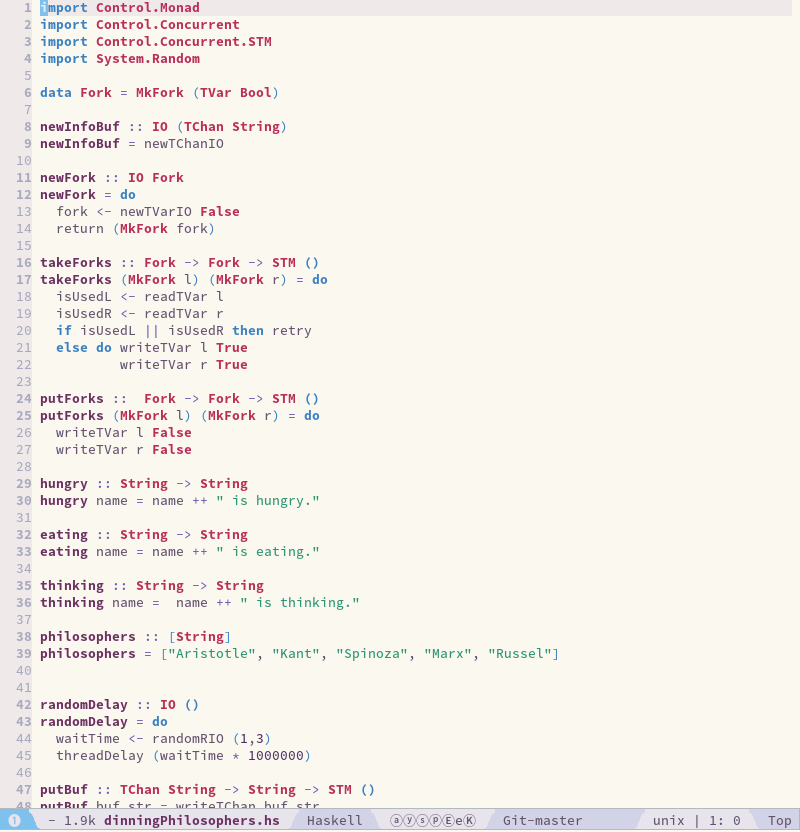
\includegraphics[scale=0.4]{dinning1}}
    \caption{Dinning Philosopher Part I}
    \label{fig:dinning1}
  \end{figure}

    \begin{figure}[H]
    \centering
    \centerline{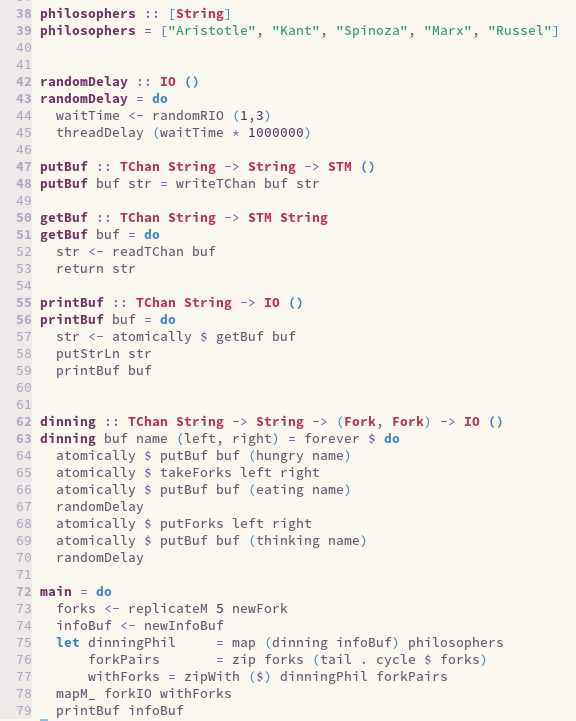
\includegraphics[scale=0.4]{dinning2}}
    \caption{Dinning Philosopher Part II}
    \label{fig:dinning2}
  \end{figure}

  


  \section{Task II.2}
  
  \begin{figure}[H]
    \centering
    \centerline{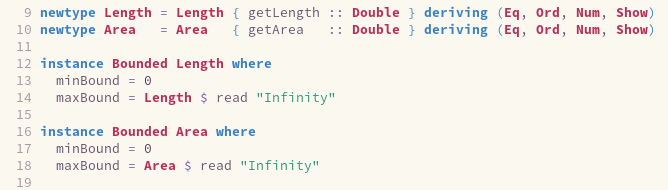
\includegraphics[scale=0.4]{StatsBonusBound}}
    \caption{newtype Bounded}
    \label{fig:bounded}
  \end{figure}

  
  \begin{figure}[H]

    \begin{minipage}[b]{0.48\linewidth}
      \centering
      \centerline{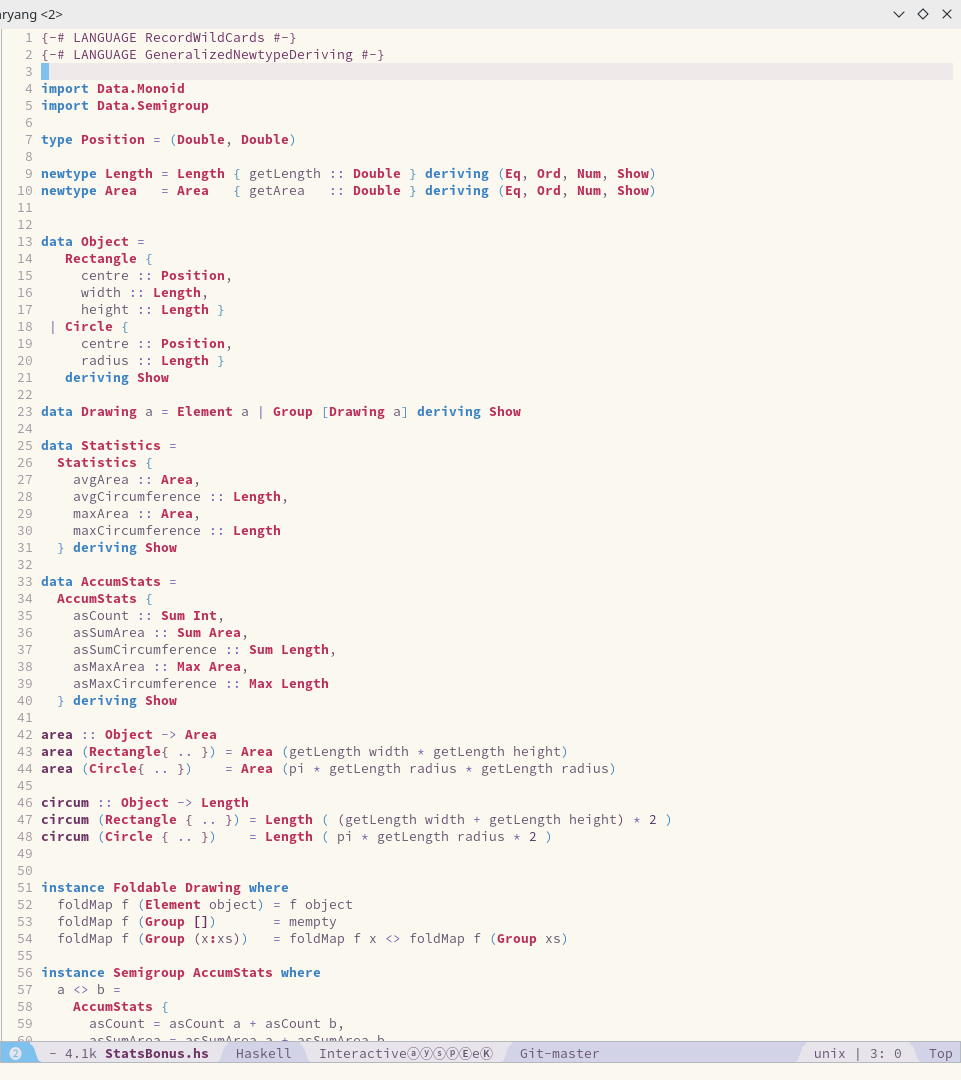
\includegraphics[width=8.0cm]{StatsBonus}}
      % \vspace{1.5cm}
      \centerline{ (a) Recursive Statistics for newtype}\medskip
    \end{minipage}
    \hfill
    \begin{minipage}[b]{0.48\linewidth}
      \centering
      \centerline{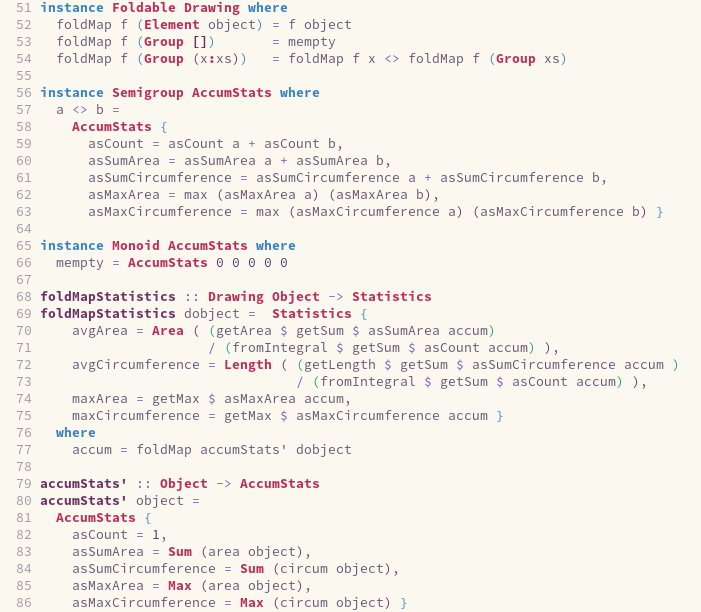
\includegraphics[width=8.0cm]{StatsBonusFoldMap}}
      % \vspace{1.5cm}
      \centerline{ (b) Statistics using foldMap for newtype}\medskip
    \end{minipage}
    % 
    \caption{TaskI.5 3}
    \label{fig:taskI.5.3}
    % 
  \end{figure}

  
\end{document}


